\section{Solution}
In this section we describe the key ideas behind our design, and the decisions we made during the design process.
\subsection{Sequential Implementation}
\subsubsection{Idea}
To implement a sequential filter we had to solve a number of problems. In between each data input, we have to do 32 multiply accumulate operations. Therefore we have to buffer the latest 32 input values in an array \texttt{data}, in which the 0th index contains $x(i)$ and the last value is $x(i -31)$. This can be seen at the top of figure ~\ref{fig:architecture}. So in each step, the new data value is supplied to \texttt{data}[0], and for all $1 \leq i \leq 31$ the value of \texttt{data}[$i$-1] is copied to \texttt{data}[$i$]. An alternative solution would be to create a ring buffer, in which we supply the input value to the $(n\bmod 32)$-th slot of \texttt{data}. We decided not to use this approach, because it would require an extra register to point to the latest variable, and an extra multiplexer to index the input wires of the array.\\
After the $n^{th}$ input is supplied we need to calculate $y(n)=\Sigma_{0\leq i \leq 31}(h(i)\cdot x(n-i))$. In our design this corresponds to $\Sigma_{0 \leq i \leq 31}(data[i] * h\_in[i])$. This is done in the bottom part of  figure ~\ref{fig:architecture}. We decided to pipeline the multiply and accumulate, in order to lower the maximum period and thereby raise the sample frequency.

\begin{figure}
\begin{center}
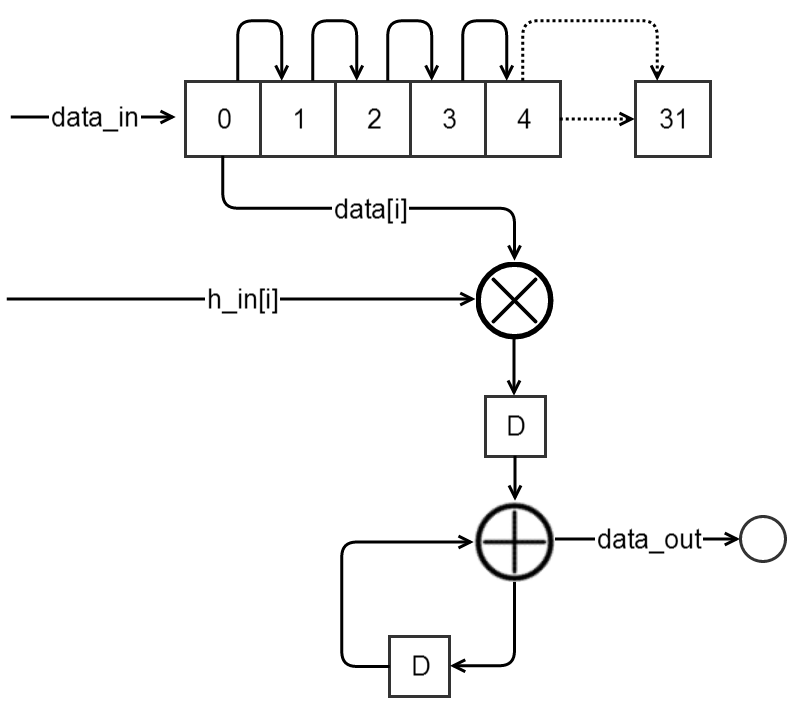
\includegraphics[width=0.6\textwidth]{images/architecture.png}
\caption{Architecture diagram of the sequential FIR filter.}
\label{fig:architecture}
\end{center}
\end{figure}

\subsubsection{Implementation}
In this section we will explain functional correctness of our code. The Verilog source code of our filter can be found in section ~\ref{sec:source1}. \\
\\
\centerline{reg [0:5] stage;}\\
\\
This declares a counter for the stage we are in. There are 32 stages during processing, and an extra state in between, which makes 33 stages. We need 6 bits to address this.\\
\\
\centerline{reg signed [0:DWIDTH-1] in [0:NR\_STAGES-1];}\\
\\
Our buffer array has words of size \texttt{DWIDTH}. It has length 32, generalized as \texttt{NR\_STAGES}.\\
\\
\centerline{reg signed [0:DDWIDTH-1] sum;}\\
\centerline{reg signed [0:DDWIDTH-1] acc;}\\
\\
The register  \texttt{sum} contains the part of the filter that has already been processed in a stage,  \texttt{acc} is the output of the multiplier. In each stage,  \texttt{acc} is added to  \texttt{sum}. They have double precision to prevent overflows.
\begin{center}
\parbox{8cm}{
 in[0] $<=$ data\_in; \\
for (i = 0; i $<$ NR\_STAGES - 1; i = i + 1) \\
begin \\
in[i + 1] $<=$ in[i]; \\
end \\
}
\end{center}
The new signal value is assigned to index 0 of the data array, the other values are moved to the next index.
\begin{center}
\parbox{10cm}{
if (stage == NR\_STAGES)\\
begin\\
\phantom{aaaa}req\_in\_buf $<=$ 1;\\
\phantom{aaaa}req\_out\_buf $<=$ 1;\\
\phantom{aaaa}out $<=$ sum + acc;\\
\phantom{aaaa}stage $<=$ 0;\\
end\\
else\\
begin\\
\phantom{aaaa}acc $<=$ (in[stage] * \$signed(h\_in[stage*DWIDTH+:DWIDTH])) $>>$ DWIDTH;\\
\phantom{aaaa}sum $<=$ sum + acc;\\
\phantom{aaaa}stage $<=$ stage + 1;\\
end\\
}
\end{center}
In each $i^{th}$ of the 32 stages we calculate \texttt{sum += h[i] * data[i]}. Because we pipelined the filter, the multiply and accumulate have a delay between them. When we finished the last stage, we signal that the system is ready to send output and receive new input.
\subsection{Strength Reduced }
\subsubsection{Idea}
todo
\subsubsection{Implementation}
todo

